%
%===============>>  ГРУППА 10-1 МОДУЛЬ 5  <<=============
%
\setmodule{5}

%BEGIN_FOLD % ====>>_____ Занятие 1 _____<<====
\begin{class}[number=1]
	\begin{listofex}
		\item
		\begin{minipage}[t]{\bodywidth}
			На рисунке изображён график функции вида \[ f(x)=ax+|bx+c|+d, \] где \(a, b, c, d\) --- целые числа. Найдите корень уравнения \(bx+c=0\).
		\end{minipage}
		\hspace{0.02\linewidth}
		\begin{minipage}[t]{\picwidth}
			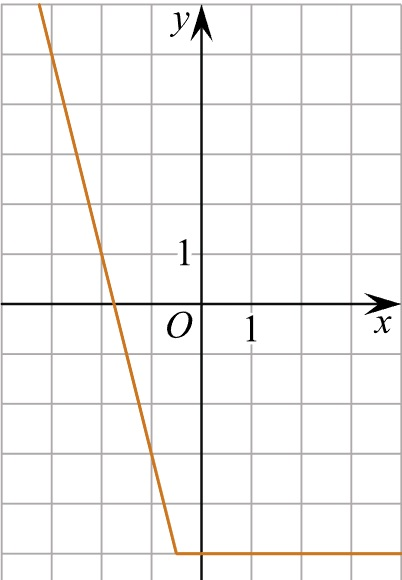
\includegraphics[align=t, width=\linewidth]{\picpath/G101M4H2-6}
		\end{minipage}
		\item
		\begin{minipage}[t]{\bodywidth}
			На рисунке изображён график функции вида \[ f(x)=ax-|bx+c|+d, \] где \(a, b, c, d\) --- целые числа. Найдите корень уравнения \(ax=d\).
		\end{minipage}
		\hspace{0.02\linewidth}
		\begin{minipage}[t]{\picwidth}
			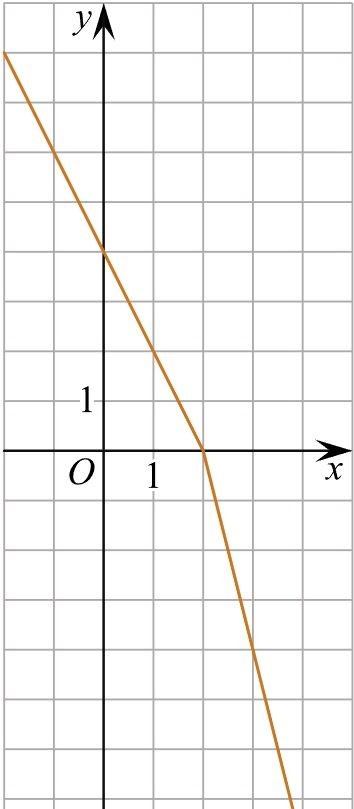
\includegraphics[align=t, width=\linewidth]{\picpath/G101M4H2-7}
		\end{minipage}
		\item
		\begin{minipage}[t]{\bodywidth}
			На рисунке изображён график функции вида \[ f(x)=ax+|bx+c|+d, \] где числа \(a, b, c, d\) --- целые. Найдите корень уравнения \(-ax-3d=10\).
		\end{minipage}
		\hspace{0.02\linewidth}
		\begin{minipage}[t]{\picwidth}
			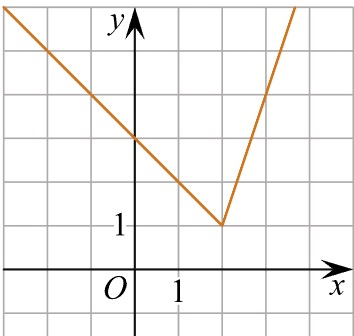
\includegraphics[align=t, width=\linewidth]{\picpath/G101M4C5-7}
		\end{minipage}
				\item
		\begin{minipage}[t]{\bodywidth}
			На рисунке изображён график функции вида \[ f(x)=ax+|bx+c|+d, \] где числа \(a, b, c, d\) --- целые. Найдите корень уравнения \(bx+2c=1\).
		\end{minipage}
		\hspace{0.02\linewidth}
		\begin{minipage}[t]{\picwidth}
			\includegraphics[align=t, width=\linewidth]{\picpath/G101M4L7-6}
		\end{minipage}
		\item Два велосипедиста одновременно отправляются в \( 60 \)-километровый пробег. Первый едет со скоростью на \( 10 \) км/ч большей, чем второй, и прибывает к финишу на \( 3 \) часа раньше второго. Найдите скорость велосипедиста, пришедшего к финишу вторым.
	\end{listofex}
\end{class}
%END_FOLD

%BEGIN_FOLD % ====>>_____ Занятие 2 _____<<====
\begin{class}[number=2]
	\begin{listofex}
		\item Занятие 2
	\end{listofex}
\end{class}
%END_FOLD

%BEGIN_FOLD % ====>>_____ Занятие 3 _____<<====
\begin{class}[number=3]
	\begin{listofex}
		\item Занятие 3
	\end{listofex}
\end{class}
%END_FOLD

%BEGIN_FOLD % ====>>_____ Занятие 4 _____<<====
\begin{class}[number=4]
	\begin{listofex}
		\item Занятие 4
	\end{listofex}
\end{class}
%END_FOLD

%BEGIN_FOLD % ====>>_____ Занятие 5 _____<<====
\begin{class}[number=5]
	\begin{listofex}
		\item Занятие 5
	\end{listofex}
\end{class}
%END_FOLD

%BEGIN_FOLD % ====>>_____ Занятие 6 _____<<====
\begin{class}[number=6]
	\begin{listofex}
		\item Занятие 6
	\end{listofex}
\end{class}
%END_FOLD

%BEGIN_FOLD % ====>>_____ Занятие 7 _____<<====
\begin{class}[number=7]
	\begin{listofex}
		\item Занятие 7
	\end{listofex}
\end{class}
%END_FOLD

%BEGIN_FOLD % ====>>_ Домашняя работа 1 _<<====
\begin{homework}[number=1]
	\begin{listofex}
		\item ДЗ 1
	\end{listofex}
\end{homework}
%END_FOLD

%BEGIN_FOLD % ====>>_ Домашняя работа 2 _<<====
\begin{homework}[number=2]
	\begin{listofex}
		\item ДЗ 2
	\end{listofex}
\end{homework}
%END_FOLD

%BEGIN_FOLD % ====>>_ Домашняя работа 3 _<<====
\begin{homework}[number=3]
	\begin{listofex}
		\item ДЗ 3
	\end{listofex}
\end{homework}
%END_FOLD

%BEGIN_FOLD % ====>>_ Проверочная работа _<<====
\begin{exam}
	\begin{listofex}
		\item Проверочная работа
	\end{listofex}
\end{exam}
%END_FOLD
